% Options for packages loaded elsewhere
\PassOptionsToPackage{unicode}{hyperref}
\PassOptionsToPackage{hyphens}{url}
%
\documentclass[
]{article}
\usepackage{lmodern}
\usepackage{amssymb,amsmath}
\usepackage{ifxetex,ifluatex}
\ifnum 0\ifxetex 1\fi\ifluatex 1\fi=0 % if pdftex
  \usepackage[T1]{fontenc}
  \usepackage[utf8]{inputenc}
  \usepackage{textcomp} % provide euro and other symbols
\else % if luatex or xetex
  \usepackage{unicode-math}
  \defaultfontfeatures{Scale=MatchLowercase}
  \defaultfontfeatures[\rmfamily]{Ligatures=TeX,Scale=1}
\fi
% Use upquote if available, for straight quotes in verbatim environments
\IfFileExists{upquote.sty}{\usepackage{upquote}}{}
\IfFileExists{microtype.sty}{% use microtype if available
  \usepackage[]{microtype}
  \UseMicrotypeSet[protrusion]{basicmath} % disable protrusion for tt fonts
}{}
\makeatletter
\@ifundefined{KOMAClassName}{% if non-KOMA class
  \IfFileExists{parskip.sty}{%
    \usepackage{parskip}
  }{% else
    \setlength{\parindent}{0pt}
    \setlength{\parskip}{6pt plus 2pt minus 1pt}}
}{% if KOMA class
  \KOMAoptions{parskip=half}}
\makeatother
\usepackage{xcolor}
\IfFileExists{xurl.sty}{\usepackage{xurl}}{} % add URL line breaks if available
\IfFileExists{bookmark.sty}{\usepackage{bookmark}}{\usepackage{hyperref}}
\hypersetup{
  pdftitle={Running a DWBA simulation ensemble for Calanus finmarchicus in Tromsøflaket},
  pdfauthor={Muriel Dunn},
  hidelinks,
  pdfcreator={LaTeX via pandoc}}
\urlstyle{same} % disable monospaced font for URLs
\usepackage[margin=1in]{geometry}
\usepackage{color}
\usepackage{fancyvrb}
\newcommand{\VerbBar}{|}
\newcommand{\VERB}{\Verb[commandchars=\\\{\}]}
\DefineVerbatimEnvironment{Highlighting}{Verbatim}{commandchars=\\\{\}}
% Add ',fontsize=\small' for more characters per line
\usepackage{framed}
\definecolor{shadecolor}{RGB}{248,248,248}
\newenvironment{Shaded}{\begin{snugshade}}{\end{snugshade}}
\newcommand{\AlertTok}[1]{\textcolor[rgb]{0.94,0.16,0.16}{#1}}
\newcommand{\AnnotationTok}[1]{\textcolor[rgb]{0.56,0.35,0.01}{\textbf{\textit{#1}}}}
\newcommand{\AttributeTok}[1]{\textcolor[rgb]{0.77,0.63,0.00}{#1}}
\newcommand{\BaseNTok}[1]{\textcolor[rgb]{0.00,0.00,0.81}{#1}}
\newcommand{\BuiltInTok}[1]{#1}
\newcommand{\CharTok}[1]{\textcolor[rgb]{0.31,0.60,0.02}{#1}}
\newcommand{\CommentTok}[1]{\textcolor[rgb]{0.56,0.35,0.01}{\textit{#1}}}
\newcommand{\CommentVarTok}[1]{\textcolor[rgb]{0.56,0.35,0.01}{\textbf{\textit{#1}}}}
\newcommand{\ConstantTok}[1]{\textcolor[rgb]{0.00,0.00,0.00}{#1}}
\newcommand{\ControlFlowTok}[1]{\textcolor[rgb]{0.13,0.29,0.53}{\textbf{#1}}}
\newcommand{\DataTypeTok}[1]{\textcolor[rgb]{0.13,0.29,0.53}{#1}}
\newcommand{\DecValTok}[1]{\textcolor[rgb]{0.00,0.00,0.81}{#1}}
\newcommand{\DocumentationTok}[1]{\textcolor[rgb]{0.56,0.35,0.01}{\textbf{\textit{#1}}}}
\newcommand{\ErrorTok}[1]{\textcolor[rgb]{0.64,0.00,0.00}{\textbf{#1}}}
\newcommand{\ExtensionTok}[1]{#1}
\newcommand{\FloatTok}[1]{\textcolor[rgb]{0.00,0.00,0.81}{#1}}
\newcommand{\FunctionTok}[1]{\textcolor[rgb]{0.00,0.00,0.00}{#1}}
\newcommand{\ImportTok}[1]{#1}
\newcommand{\InformationTok}[1]{\textcolor[rgb]{0.56,0.35,0.01}{\textbf{\textit{#1}}}}
\newcommand{\KeywordTok}[1]{\textcolor[rgb]{0.13,0.29,0.53}{\textbf{#1}}}
\newcommand{\NormalTok}[1]{#1}
\newcommand{\OperatorTok}[1]{\textcolor[rgb]{0.81,0.36,0.00}{\textbf{#1}}}
\newcommand{\OtherTok}[1]{\textcolor[rgb]{0.56,0.35,0.01}{#1}}
\newcommand{\PreprocessorTok}[1]{\textcolor[rgb]{0.56,0.35,0.01}{\textit{#1}}}
\newcommand{\RegionMarkerTok}[1]{#1}
\newcommand{\SpecialCharTok}[1]{\textcolor[rgb]{0.00,0.00,0.00}{#1}}
\newcommand{\SpecialStringTok}[1]{\textcolor[rgb]{0.31,0.60,0.02}{#1}}
\newcommand{\StringTok}[1]{\textcolor[rgb]{0.31,0.60,0.02}{#1}}
\newcommand{\VariableTok}[1]{\textcolor[rgb]{0.00,0.00,0.00}{#1}}
\newcommand{\VerbatimStringTok}[1]{\textcolor[rgb]{0.31,0.60,0.02}{#1}}
\newcommand{\WarningTok}[1]{\textcolor[rgb]{0.56,0.35,0.01}{\textbf{\textit{#1}}}}
\usepackage{graphicx,grffile}
\makeatletter
\def\maxwidth{\ifdim\Gin@nat@width>\linewidth\linewidth\else\Gin@nat@width\fi}
\def\maxheight{\ifdim\Gin@nat@height>\textheight\textheight\else\Gin@nat@height\fi}
\makeatother
% Scale images if necessary, so that they will not overflow the page
% margins by default, and it is still possible to overwrite the defaults
% using explicit options in \includegraphics[width, height, ...]{}
\setkeys{Gin}{width=\maxwidth,height=\maxheight,keepaspectratio}
% Set default figure placement to htbp
\makeatletter
\def\fps@figure{htbp}
\makeatother
\setlength{\emergencystretch}{3em} % prevent overfull lines
\providecommand{\tightlist}{%
  \setlength{\itemsep}{0pt}\setlength{\parskip}{0pt}}
\setcounter{secnumdepth}{-\maxdimen} % remove section numbering

\title{Running a DWBA simulation ensemble for Calanus finmarchicus in
Tromsøflaket}
\author{Muriel Dunn}
\date{2020-09-09}

\begin{document}
\maketitle

\begin{verbatim}
## Warning: replacing previous import 'shiny::runExample' by 'shinyjs::runExample'
## when loading 'ZooScatR'
\end{verbatim}

This document shows how I used the DWBA model within the ZooScatR
package to run model ensembles to calculate the target spectra of
Calanus finmarchicus in Tromsøflaket.

\hypertarget{first-iteration}{%
\subsection{First iteration}\label{first-iteration}}

I have entered the parameter files for an ``average'' Calanus
finmarchicus in the config\_calanusFinCV.dat. Let's check it out to see
if it makes sense for TS spectra, backscattering cross-section and TS vs
ka (to check for Rayleigh to geometric scattering.)

\begin{Shaded}
\begin{Highlighting}[]
\NormalTok{fname <-}\StringTok{ }\KeywordTok{paste0}\NormalTok{(}\StringTok{"/Users/mbd/phd/ZooScatStuff/config_EukrohniaHamata.dat"}\NormalTok{) }\CommentTok{#Location of the parameters file}

\NormalTok{para =}\StringTok{ }\KeywordTok{read_para}\NormalTok{(fname) }\CommentTok{#Read parameters file}
\CommentTok{#Create list with soundspeed info}
\NormalTok{misc <-}\StringTok{ }\KeywordTok{list}\NormalTok{(}\DataTypeTok{cw=}\DecValTok{1486}\NormalTok{)}
\CommentTok{#Run DWBA based on config file}
\NormalTok{res_TS <-}\StringTok{ }\KeywordTok{bscat}\NormalTok{(}\DataTypeTok{para=}\NormalTok{para, }\DataTypeTok{misc=}\NormalTok{misc) }\CommentTok{#Target strength vs Frequency}
\NormalTok{res_TS}\OperatorTok{$}\NormalTok{rplot }\CommentTok{#Show the result plot}
\end{Highlighting}
\end{Shaded}

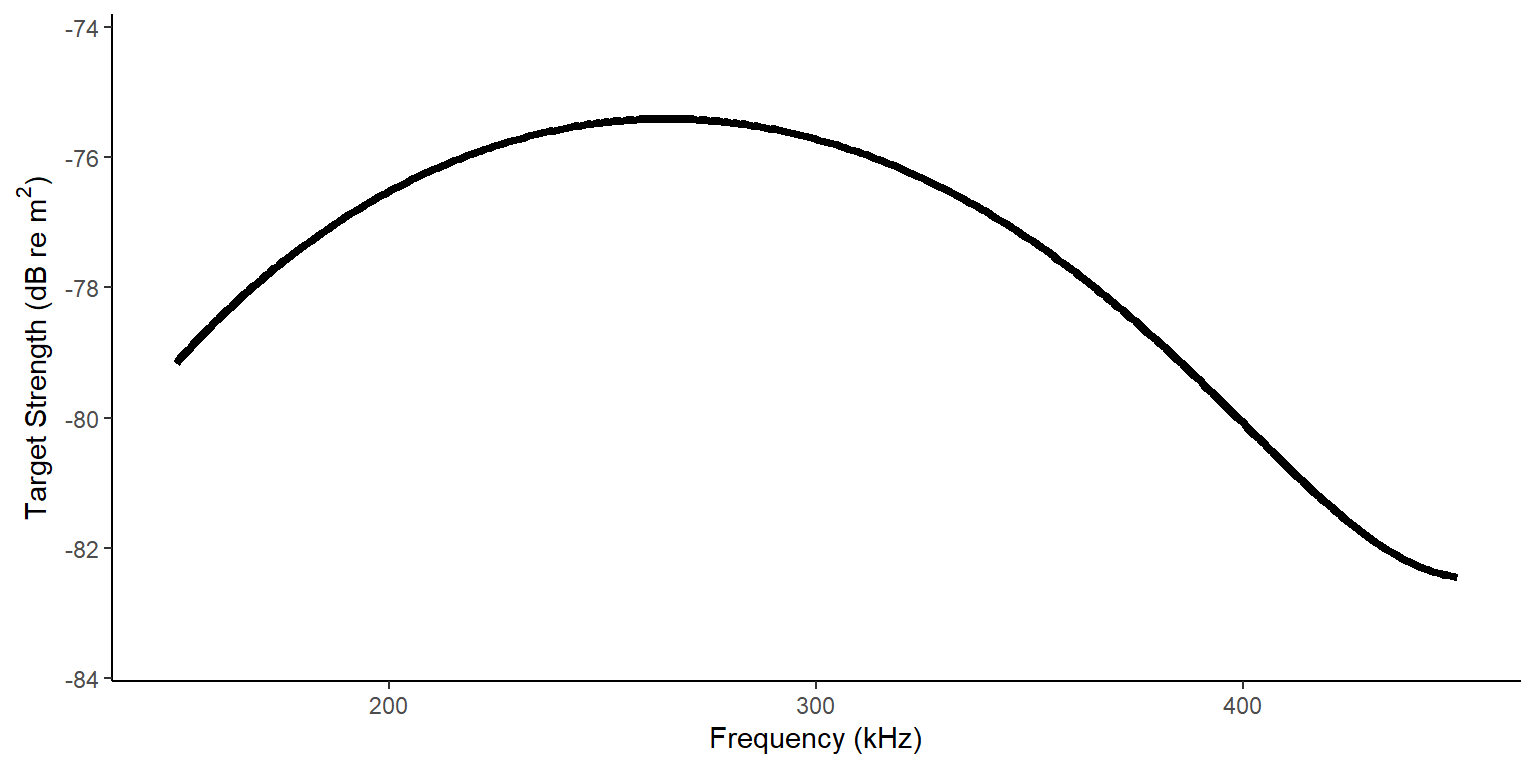
\includegraphics{runDwbaEnsemble_files/figure-latex/unnamed-chunk-1-1.pdf}

\begin{Shaded}
\begin{Highlighting}[]


\CommentTok{#cross-section vs frequency}
\NormalTok{para}\OperatorTok{$}\NormalTok{simu}\OperatorTok{$}\NormalTok{out_indx <-}\StringTok{ }\DecValTok{2} \CommentTok{#Set output variable to cross section}
\CommentTok{#Run DWBA based on config file}
\NormalTok{res_sig <-}\StringTok{ }\KeywordTok{bscat}\NormalTok{(}\DataTypeTok{para=}\NormalTok{para, }\DataTypeTok{misc=}\NormalTok{misc)}
\NormalTok{res_sig}\OperatorTok{$}\NormalTok{rplot }\CommentTok{#Show the result plot}
\end{Highlighting}
\end{Shaded}

\includegraphics{runDwbaEnsemble_files/figure-latex/unnamed-chunk-1-2.pdf}

\begin{Shaded}
\begin{Highlighting}[]

\CommentTok{#Backscattering amplitude vs ka (Wavenumber x width)}
\NormalTok{para}\OperatorTok{$}\NormalTok{simu}\OperatorTok{$}\NormalTok{out_indx <-}\StringTok{ }\DecValTok{3} \CommentTok{#Set output to Target Strength}
\NormalTok{para}\OperatorTok{$}\NormalTok{simu}\OperatorTok{$}\NormalTok{var_indx <-}\StringTok{ }\DecValTok{3} \CommentTok{#Set output variable to ka}
\NormalTok{para}\OperatorTok{$}\NormalTok{simu}\OperatorTok{$}\NormalTok{var0 =}\StringTok{ }\FloatTok{0.1} \CommentTok{#simulate from ka=0 }
\NormalTok{para}\OperatorTok{$}\NormalTok{simu}\OperatorTok{$}\NormalTok{var1 =}\StringTok{ }\DecValTok{10} \CommentTok{#...to ka=10}
\CommentTok{#Run DWBA based on config file}
\NormalTok{res <-}\StringTok{ }\KeywordTok{bscat}\NormalTok{(}\DataTypeTok{para=}\NormalTok{para, }\DataTypeTok{misc=}\NormalTok{misc)}
\NormalTok{res}\OperatorTok{$}\NormalTok{rplot }\CommentTok{#Show the result plot}
\end{Highlighting}
\end{Shaded}

\includegraphics{runDwbaEnsemble_files/figure-latex/unnamed-chunk-1-3.pdf}

\hypertarget{simulations}{%
\subsection{SIMULATIONS!}\label{simulations}}

\begin{Shaded}
\begin{Highlighting}[]

\NormalTok{Species_name =}\StringTok{ "CalanusFinCV"}
\NormalTok{Species_name =}\StringTok{ "EuphausiaceaFurcilia"}
\NormalTok{Species_name =}\StringTok{ "EukrohniaHamata"}

\NormalTok{fname <-}\StringTok{ }\KeywordTok{paste0}\NormalTok{(}\StringTok{"/Users/mbd/phd/ZooScatStuff/config_"}\NormalTok{, Species_name, }\StringTok{".dat"}\NormalTok{)}
\NormalTok{para =}\StringTok{ }\KeywordTok{read_para}\NormalTok{(fname) }\CommentTok{#Read parameters file}

\CommentTok{#make a length simulation}
\NormalTok{para}\OperatorTok{$}\NormalTok{shape}\OperatorTok{$}\NormalTok{ave_flag <-}\StringTok{ }\DecValTok{1}
\CommentTok{#make an orientation simulation}
\NormalTok{para}\OperatorTok{$}\NormalTok{orient}\OperatorTok{$}\NormalTok{ave_flag <-}\StringTok{ }\DecValTok{1}

\NormalTok{para}\OperatorTok{$}\NormalTok{simu}\OperatorTok{$}\NormalTok{var0 =}\StringTok{ }\DecValTok{180} \CommentTok{#simulate from 180 }
\NormalTok{para}\OperatorTok{$}\NormalTok{simu}\OperatorTok{$}\NormalTok{var1 =}\StringTok{ }\DecValTok{450} \CommentTok{#...to 450 kHz}
\NormalTok{para}\OperatorTok{$}\NormalTok{simu}\OperatorTok{$}\NormalTok{ni =}\StringTok{ }\DecValTok{200} \CommentTok{#reduce the number of elements and frequencies to improve speed}
\NormalTok{para}\OperatorTok{$}\NormalTok{simu}\OperatorTok{$}\NormalTok{n =}\StringTok{ }\DecValTok{483}

\CommentTok{#Create list with sound speed info}
\NormalTok{misc <-}\StringTok{ }\KeywordTok{list}\NormalTok{(}\DataTypeTok{cw=}\DecValTok{1486}\NormalTok{)}



\NormalTok{res <-}\StringTok{ }\KeywordTok{bscat}\NormalTok{(}\DataTypeTok{para=}\NormalTok{para, }\DataTypeTok{misc=}\NormalTok{misc, }\DataTypeTok{simOut =} \OtherTok{TRUE}\NormalTok{, }\DataTypeTok{nang=}\DecValTok{350}\NormalTok{, }\DataTypeTok{nl=}\DecValTok{350}\NormalTok{) }\CommentTok{#Target strength vs Frequency}
\end{Highlighting}
\end{Shaded}

\hypertarget{plotting-the-results}{%
\subsection{Plotting the results}\label{plotting-the-results}}

\begin{Shaded}
\begin{Highlighting}[]
\NormalTok{o_sim =}\StringTok{ }\KeywordTok{melt}\NormalTok{(res}\OperatorTok{$}\NormalTok{ysim)}
\NormalTok{o_sim}\OperatorTok{$}\NormalTok{theta =}\StringTok{ }\NormalTok{res}\OperatorTok{$}\NormalTok{ang[o_sim}\OperatorTok{$}\NormalTok{Var2]}
\NormalTok{o_sim}\OperatorTok{$}\NormalTok{Frequency =}\StringTok{ }\NormalTok{res}\OperatorTok{$}\NormalTok{var[o_sim}\OperatorTok{$}\NormalTok{Var1]}
\NormalTok{o_sim=o_sim[,}\DecValTok{3}\OperatorTok{:}\KeywordTok{ncol}\NormalTok{(o_sim)]}
\KeywordTok{names}\NormalTok{(o_sim)[}\DecValTok{1}\NormalTok{] <-}\StringTok{ 'TS'}

\NormalTok{mTS =}\StringTok{ }\KeywordTok{data.frame}\NormalTok{(}\DataTypeTok{Frequency=}\NormalTok{res}\OperatorTok{$}\NormalTok{var,}\DataTypeTok{TS=}\NormalTok{res}\OperatorTok{$}\NormalTok{y)}

\KeywordTok{ggplot}\NormalTok{()}\OperatorTok{+}\KeywordTok{geom_line}\NormalTok{(}\DataTypeTok{data=}\NormalTok{o_sim, }\KeywordTok{aes}\NormalTok{(}\DataTypeTok{x =}\NormalTok{ Frequency, }\DataTypeTok{y=}\NormalTok{TS, }\DataTypeTok{group=}\NormalTok{theta),}\DataTypeTok{lty=}\DecValTok{2}\NormalTok{, }\DataTypeTok{lwd=}\FloatTok{0.5}\NormalTok{, }\DataTypeTok{alpha=}\FloatTok{0.4}\NormalTok{)}\OperatorTok{+}
\StringTok{  }\KeywordTok{geom_line}\NormalTok{(}\DataTypeTok{data=}\NormalTok{mTS, }\KeywordTok{aes}\NormalTok{(}\DataTypeTok{x=}\NormalTok{Frequency, }\DataTypeTok{y=}\NormalTok{TS), }\DataTypeTok{lty=}\DecValTok{1}\NormalTok{, }\DataTypeTok{lwd=}\DecValTok{2}\NormalTok{)}\OperatorTok{+}
\StringTok{  }\KeywordTok{theme_classic}\NormalTok{()}\OperatorTok{+}
\StringTok{  }\KeywordTok{theme}\NormalTok{(}\DataTypeTok{text=}\KeywordTok{element_text}\NormalTok{(}\DataTypeTok{size=}\DecValTok{14}\NormalTok{))}\OperatorTok{+}
\StringTok{  }\KeywordTok{ggtitle}\NormalTok{(Species_name)}
\end{Highlighting}
\end{Shaded}

\includegraphics{runDwbaEnsemble_files/figure-latex/plots_osim-1.pdf}

\begin{Shaded}
\begin{Highlighting}[]

\KeywordTok{ggplot}\NormalTok{(}\DataTypeTok{data=}\NormalTok{o_sim, }\KeywordTok{aes}\NormalTok{(}\DataTypeTok{x=}\NormalTok{Frequency, }\DataTypeTok{y=}\NormalTok{theta, }\DataTypeTok{fill=}\NormalTok{TS))}\OperatorTok{+}
\StringTok{  }\KeywordTok{geom_raster}\NormalTok{()}\OperatorTok{+}
\StringTok{  }\KeywordTok{scale_fill_viridis_c}\NormalTok{()}\OperatorTok{+}
\StringTok{  }\KeywordTok{scale_y_continuous}\NormalTok{(}\DataTypeTok{expand=}\KeywordTok{c}\NormalTok{(}\DecValTok{0}\NormalTok{,}\DecValTok{0}\NormalTok{))}\OperatorTok{+}
\StringTok{  }\KeywordTok{scale_x_continuous}\NormalTok{(}\DataTypeTok{expand=}\KeywordTok{c}\NormalTok{(}\DecValTok{0}\NormalTok{,}\DecValTok{0}\NormalTok{))}\OperatorTok{+}
\StringTok{  }\KeywordTok{theme_classic}\NormalTok{()}\OperatorTok{+}\KeywordTok{theme}\NormalTok{(}\DataTypeTok{text=}\KeywordTok{element_text}\NormalTok{(}\DataTypeTok{size=}\DecValTok{14}\NormalTok{))}\OperatorTok{+}
\StringTok{  }\KeywordTok{ggtitle}\NormalTok{(Species_name)}
\end{Highlighting}
\end{Shaded}

\includegraphics{runDwbaEnsemble_files/figure-latex/plots_osim-2.pdf}

\hypertarget{length-simulations}{%
\subsubsection{Length simulations}\label{length-simulations}}

\begin{Shaded}
\begin{Highlighting}[]
\NormalTok{l_sim =}\StringTok{  }\KeywordTok{melt}\NormalTok{(res}\OperatorTok{$}\NormalTok{ysimL)}
\NormalTok{l_sim}\OperatorTok{$}\NormalTok{Length =}\StringTok{ }\NormalTok{res}\OperatorTok{$}\NormalTok{L[l_sim}\OperatorTok{$}\NormalTok{Var2]}
\NormalTok{l_sim}\OperatorTok{$}\NormalTok{Frequency =}\StringTok{ }\NormalTok{res}\OperatorTok{$}\NormalTok{var[l_sim}\OperatorTok{$}\NormalTok{Var1]}
\NormalTok{l_sim=l_sim[,}\DecValTok{3}\OperatorTok{:}\KeywordTok{ncol}\NormalTok{(l_sim)]}
\KeywordTok{names}\NormalTok{(l_sim)[}\DecValTok{1}\NormalTok{] <-}\StringTok{ 'TS'}

\KeywordTok{ggplot}\NormalTok{()}\OperatorTok{+}\KeywordTok{geom_line}\NormalTok{(}\DataTypeTok{data=}\NormalTok{l_sim, }\KeywordTok{aes}\NormalTok{(}\DataTypeTok{x =}\NormalTok{ Frequency, }\DataTypeTok{y=}\NormalTok{TS, }\DataTypeTok{group=}\NormalTok{Length),}\DataTypeTok{lty=}\DecValTok{2}\NormalTok{, }\DataTypeTok{lwd=}\FloatTok{0.5}\NormalTok{, }\DataTypeTok{alpha=}\FloatTok{0.4}\NormalTok{)}\OperatorTok{+}
\StringTok{  }\KeywordTok{geom_line}\NormalTok{(}\DataTypeTok{data=}\NormalTok{mTS, }\KeywordTok{aes}\NormalTok{(}\DataTypeTok{x=}\NormalTok{Frequency, }\DataTypeTok{y=}\NormalTok{TS), }\DataTypeTok{lty=}\DecValTok{1}\NormalTok{, }\DataTypeTok{lwd=}\DecValTok{2}\NormalTok{)}\OperatorTok{+}\KeywordTok{theme_classic}\NormalTok{()}\OperatorTok{+}\KeywordTok{theme}\NormalTok{(}\DataTypeTok{text=}\KeywordTok{element_text}\NormalTok{(}\DataTypeTok{size=}\DecValTok{14}\NormalTok{))}\OperatorTok{+}
\StringTok{  }\KeywordTok{ggtitle}\NormalTok{(Species_name)}
\end{Highlighting}
\end{Shaded}

\includegraphics{runDwbaEnsemble_files/figure-latex/plots_L-1.pdf}

\begin{Shaded}
\begin{Highlighting}[]



\KeywordTok{ggplot}\NormalTok{(}\DataTypeTok{data=}\NormalTok{l_sim, }\KeywordTok{aes}\NormalTok{(}\DataTypeTok{x=}\NormalTok{Frequency, }\DataTypeTok{y=}\NormalTok{Length, }\DataTypeTok{fill=}\NormalTok{TS))}\OperatorTok{+}
\StringTok{  }\KeywordTok{geom_raster}\NormalTok{()}\OperatorTok{+}
\StringTok{  }\KeywordTok{scale_fill_viridis_c}\NormalTok{()}\OperatorTok{+}
\StringTok{  }\KeywordTok{scale_y_continuous}\NormalTok{(}\DataTypeTok{expand=}\KeywordTok{c}\NormalTok{(}\DecValTok{0}\NormalTok{,}\DecValTok{0}\NormalTok{))}\OperatorTok{+}
\StringTok{  }\KeywordTok{scale_x_continuous}\NormalTok{(}\DataTypeTok{expand=}\KeywordTok{c}\NormalTok{(}\DecValTok{0}\NormalTok{,}\DecValTok{0}\NormalTok{))}\OperatorTok{+}
\StringTok{  }\KeywordTok{theme_classic}\NormalTok{()}\OperatorTok{+}\KeywordTok{theme}\NormalTok{(}\DataTypeTok{text=}\KeywordTok{element_text}\NormalTok{(}\DataTypeTok{size=}\DecValTok{14}\NormalTok{))}\OperatorTok{+}
\StringTok{  }\KeywordTok{ggtitle}\NormalTok{(Species_name)}
\end{Highlighting}
\end{Shaded}

\includegraphics{runDwbaEnsemble_files/figure-latex/plots_L-2.pdf}

\hypertarget{confidence-intervals-of-ts-spectra}{%
\subsubsection{Confidence Intervals of TS
Spectra}\label{confidence-intervals-of-ts-spectra}}

\end{document}
